\chapter{Methodology}
In this section, we present the methodology for self-supervised skeleton-based action recognition, exploring two distinct approaches to leverage the benefits of self-supervised learning: DINO with STTFormer and PSTL with ST-GCN. We will compare their performance on benchmark datasets, highlighting learning strategies, and data preprocessing. First we propose an approach inspired by the DINO framework introduced in \cite{caron2021emerging}. Unlike the original DINO, which focuses on image data, our adaptation is designed explicitly for 3D skeleton data. In the DINO framework, the self-distillation technique is applied, wherein a vision transformer is used as the teacher network. In our context, we leverage the momentum encoder of STTFormer as the teacher network, predicting its output directly. We use a standard cross-entropy loss to align the student and teacher predictions, effectively learning meaningful representations without the need for labeled data. The core idea is to utilize the STTFormer, a spatio-temporal transformer-based network, as the encoder for our self-supervised learning. The second approach we explore is the Partial Spatio-Temporal Learning (PSTL) framework, a method explicitly designed for skeleton-based action recognition. In this approach, we employ the ST-GCN architecture as the backbone.

For our experiments, we will employ the existing PSTL framework and compare it with the DINO approach. The first approach utilizes the combination of PSTL with ST-GCN as the encoder. Our second approach, which is our contribution, employs a new combination of DINO and STTFormer as an encoder. For both approaches, we adopt self-supervised learning strategies, where the model learns to make meaningful predictions from the unlabeled skeleton data. This allows us to overcome the limitations of traditional supervised methods, which rely on costly and time-consuming data annotation. During training, we employ data preprocessing techniques to prepare the skeleton data for learning. This includes normalization, joint alignment, and temporal synchronization. Additionally, we apply data augmentation to increase the diversity of the training set and enhance the robustness of the learned representations. The goal is to identify the strengths and weaknesses of each method, providing valuable insights into the application of self-supervised learning for skeleton-based action recognition.

\section{First Approach Overview: DINO \& STTFormer}
The success of the DINO framework in self-supervised learning for images, where a transformer serves as the backbone, has motivated us to explore its potential for skeleton-based action recognition. Transformers have demonstrated remarkable capabilities in learning meaningful representations from data, especially in self-supervised learning tasks. Leveraging the success of transformers in SSL, we propose to use the STTFormer as the backbone in our DINO-inspired approach. In our DINO-inspired approach, we employ two streams with the same encoder, the STTFormer. As shown in ~\ref{fig:DINO_pipeline}The architecture consists of an upper stream, representing the student, and a lower stream, acting as the teacher. The primary objective is for the student to learn good representations from the teacher. The key feature is the self-distillation technique, where the teacher network guides the learning of a student network through cross-entropy loss. 
The student learns from the gradients backpropagated through the loss function during training. However, there is a stop gradient applied to the teacher to prevent direct influence from the student's updates. Instead, the teacher learns from the exponential moving average of the student's weights, creating a smoother and more stable learning process.

The encoder in our approach utilizes spatio-temporal tuples encoding to capture both spatial and temporal relationships within the skeleton data. This encoding strategy allows the model to extract meaningful joint interactions and motion patterns essential for accurate action recognition.

\begin{figure}
	\centering
	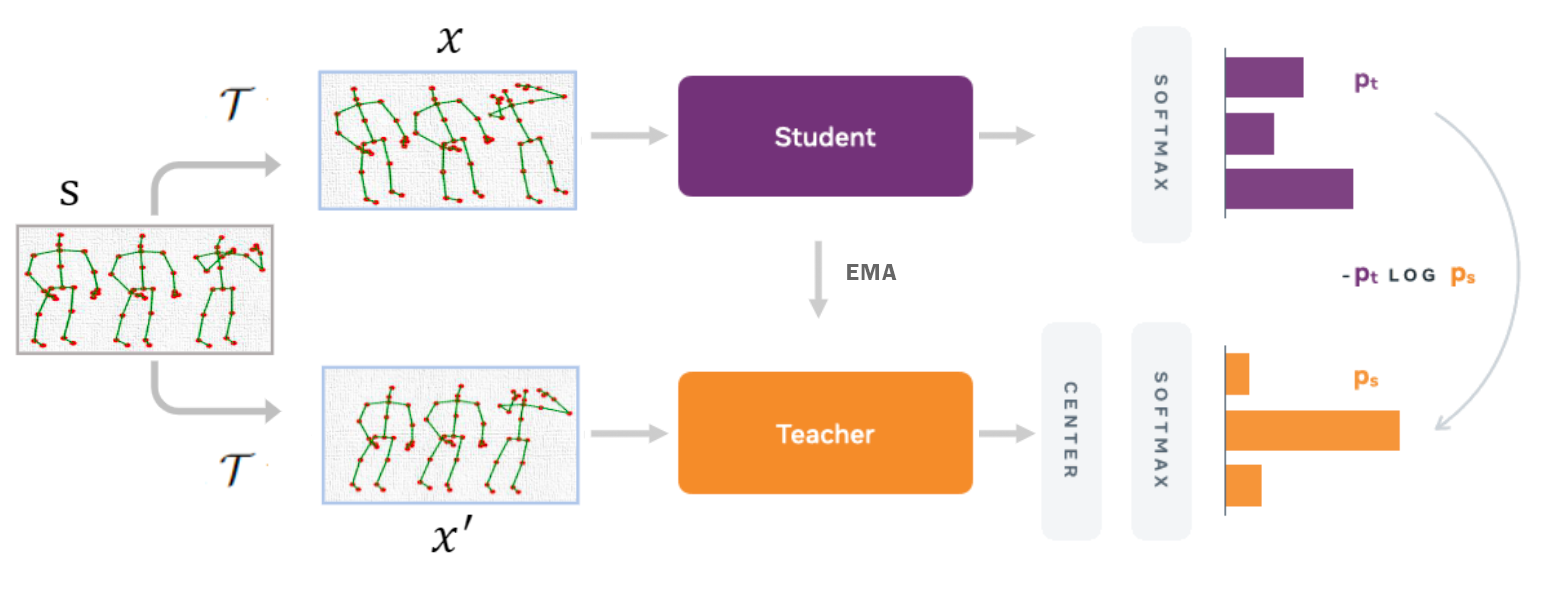
\includegraphics[width=.9\linewidth]{img/DINO_pipeline.png}
	\caption{Illustration of the DINO framework where The model passes two different random transformations (x,x') of an input image s to the student and teacher networks.}\label{fig:DINO_pipeline}
\end{figure}

In the following section, we provide a comprehensive breakdown of each component within the Spatio-Temporal Tuples Transformer. This includes detailed descriptions of self-attention mechanisms with (STTA) blocks, and Inter-Frame Feature Aggregation (IFFA). We also elaborate on positional encoding and its significance in capturing the sequential dependencies of skeleton data.

\subsection{Backbone Encoder: STTFormer}
Spatio-Temporal Tuples Transformer (STTFormer) is a novel method for skeleton-based action recognition that captures the dependencies between joints and achieves better performance on large-scale datasets. The overall architecture of STTFormer is shown in ~\ref{fig:STTFormer}. The input is a skeleton sequence with $V_0$ joints and $T_0$ frames. The sequence is divided into $T$ parts, each containing $n$ consecutive frames, for a total of $V = n * V_0$ joints. Then, a tuple encoding layer is utilized to encode each tuple data. A total of $L$ layers are stacked in the spatio-temporal tuples Transformer, and each layer is composed of Spatio-Temporal Tuples Attention (STTA) and Inter-Frame Feature Aggregation (IFFA). Finally, the obtained features are input into a global average pooling layer and a fully connected layer to obtain classification scores.

\begin{figure}
	\centering
	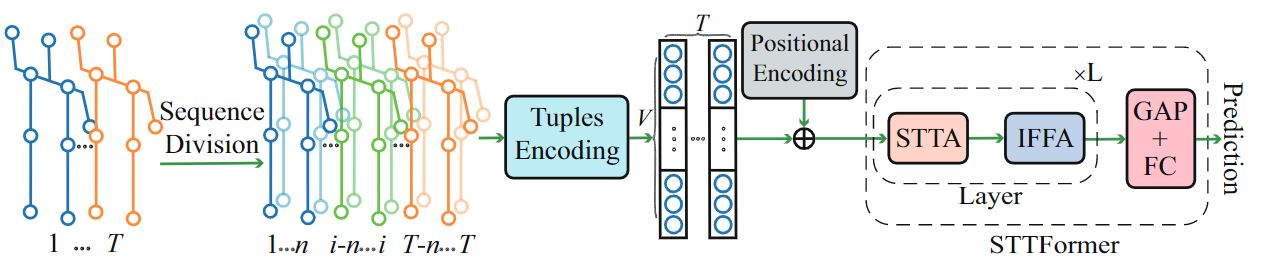
\includegraphics[width=.9\linewidth]{img/STTFormer.JPG}
	\caption{Illustration from \cite{qiu2022spatio} shows the overall architecture of the STTFormer. It consists of two main blocks: the spatio-temporal tuples encoding and  spatio-temporal tuple Transformer.}\label{fig:STTFormer}
\end{figure}


At the beginning of the Spatio-Temporal Tuples Encoding phase, each tuple is flattened into a short sequence, as the raw skeleton sequence
\(X_0 \in \mathbb{R} ^{ C_0 \times T_0 \times V_0}\) is fed to a feature mapping layer to expand the input channel to a set number $C_1$. Subsequently, the skeleton sequence is divided into $T$ non-overlapping tuples:

\begin{center}
$X = [x_1,x_2, ..., x_T], x_i \in \mathbb{R}^{C_1\times n \times V_0}$
\end{center}

Then the tuples sequence goes through a flattening layer:

\begin{center}
$X \in \mathbb{R}^{C_1 \times T \times n \times V_0} \to \mathbb{R}^{C_1 \times T \times V}$
\end{center}

where $T = T_0/n, V = n \times V_0$. Then a positional encoding strategy is used to encode the temporal and spatial information of each joint in the tuple. Specifically, each joint is represented by a vector of its 3D coordinates, and the temporal information is represented by a vector of its frame index. Then, the positional encoding is applied to each vector to capture the relative position of each joint in the tuple, as shown in ~\ref{fig:STTFormer_tuplesEncoding}. The positional encoding is defined as follows:

$$PE_{(pos,2i)} = sin(pos/10000^{2i/C_{in}})$$
$$PE_{(pos,2i+1)} = cos(pos/10000^{2i/C_{in}})$$

where $pos$ is the position of the joint in the tuple, $i$ is the index dimension of the position encoding vector, and $C_in$ is the dimension of the joint vector. The output of the encoding is defined as $X_{in}$

In the Spatio-Temporal Tuples Attention phase, a self-attention mechanism is used to capture the relationship between joints in each tuple. Specifically, a spatio-temporal tuple self-attention (STTA) module is used to extract the related features of joints in each short sequence. The STTA module is defined as follows, the encoded sequence $X_{in}$ is projected into the query $Q$, key $K$ and value $V$:


\begin{center}
$Q,K,V = Conv_{2D(1\times1)}(X_{in})$
\end{center}

Like the standard Transformer, the dot-product is used as the similarity function, the $Tanh$ function is utilized to normalize the obtained weights.

$$X_{attn}(Q,K,V) = Tanh(\frac{QK^T}{\sqrt{C}})V$$

Where $C$ denotes the number of channels of the key $K$, which can avoid excessive inner product to increase gradients stability during training. The output of the STTA module is a weighted sum of the value matrix $V$, where the weights are determined by the final attention.

\begin{figure}
	\centering
	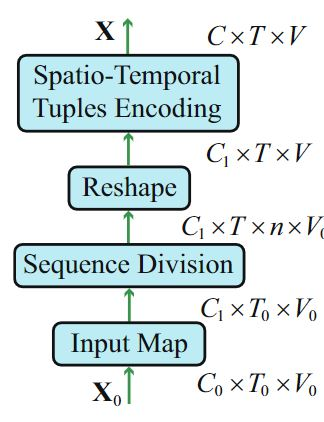
\includegraphics[width=.3\linewidth]{img/STTFormer_tuplesEncoding.JPG}
	\caption{Transformation of the input data through the spatio-temporal tuples encoding.}\label{fig:STTFormer_tuplesEncoding}
\end{figure}

To fuse the output, a feed-forward layer using $1\times1$ 2D convolution is added, resembling the transformer, as shown in ~\ref{fig:STTFormer_transoformer}.

A single action can be broken down into numerous smaller ones, such as the "long jump" which includes the "run-up," "take-off," and "landing" motions. Each tuple in the STTFormer contains a sub-action that was created by modeling a number of consecutive $n$ frames using STTA. The construction of a correlation between various sub-actions, such as "run-up," "take-off," and "landing," will aid in action recognition and aid in separating similar acts, such as high jump and long jump. In the Inter-Frame Feature Aggregation phase, a convolution operation with $k_2 \times 1$ kernel size is used to realize inter-frame feature aggregation in the temporal dimension. Specifically, the output of the STTA module is fed into a convolutional layer to aggregate the features of each joint across different frames. The IFFA operation is defined as follows:

$$X_{IFFA} = Conv_{2D(k_2 \times 1)}(X_{STTA})$$

where $X_{STTA}$ is the output of the STTA module, and $k_2$ is the kernel size. At last, the residual connections are used to stabilize network training as shown in ~\ref{fig:STTFormer_transoformer}. All outputs connected to the rest are regularized to prevent overfitting.


\begin{figure}
	\centering
	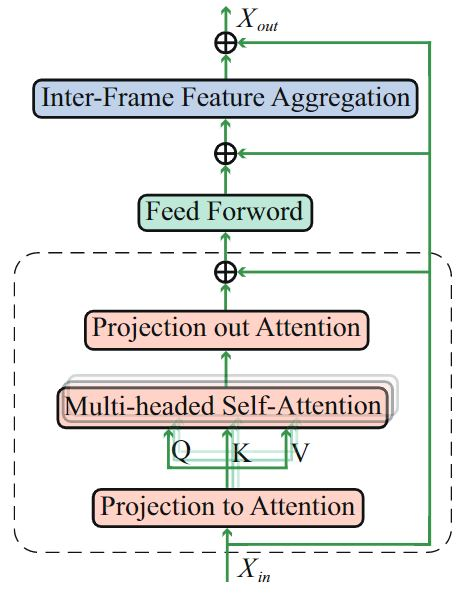
\includegraphics[width=.4\linewidth]{img/STTFormer_transoformer.JPG}
	\caption{An example of the suggested spatio-temporal tuples L of these layers make up the transformer layer, which is the whole STTFormer.}\label{fig:STTFormer_transoformer}
\end{figure}


\subsection{Learning Strategy: DINO}
In the DINO framework, the model processes two different random transformations of an input, in our method, we will pass two skeleton sequences. These transformations are passed through the student network, denoted as $g_{\theta_s}$, and the teacher network denoted as $g_{\theta_t}$. Both the student and teacher networks have identical architectures but differ in their parameters. The output of the teacher network is centered with a mean computed over the batch, resulting in a more stable and robust representation. Each network, i.e., the student and the teacher, produces a K-dimensional feature representation, denoted as $P_s$ and $P_t$, respectively, as shown in ~\ref{fig:DINO_pipeline}. These feature representations are then normalized using a softmax operation with a temperature $\tau_s$ over the feature dimension. This normalization step ensures that the features remain in a suitable range for learning and generalization:

\begin{center}
$P_s(x)^{(i)}=\frac{\exp \left(g_{\theta_s}(x)^{(i)} / \tau_s\right)}{\sum_{k=1}^K \exp \left(g_{\theta_s}(x)^{(k)} / \tau_s\right)}$,
\end{center}

The core of the DINO framework lies in the self-distillation process. With a fixed teacher, the similarity between the student and teacher features is measured using a cross-entropy loss:

\begin{center}
$\min _{\theta_s} H\left(P_t(x), P_s(x)\right)$
\end{center}

where:

\begin{center}
$H(a, b)=-a \log b$
\end{center}

More precisely, from a given skeleton sequence, a set $V$ of different skeleton augmentations is generated. This set contains two weak augmentations, $x^g_1$ and $x^g_2$ and several strong augmentations. All augmentations are passed through the student while only the weak augmentations are passed through the teacher, therefore we mimic the strategy of encouraging “local-to-global” correspondences used in images from the DINO paper. The loss then is minimized as:

$$
\min _{\theta_s} \sum_{x \in\left\{x_1^g, x_2^g\right\}} \sum_{\substack{x^{\prime} \in V \\ x^{\prime} \neq x}} H\left(P_t(x), P_s\left(x^{\prime}\right)\right)
$$

This loss function drives the student to learn meaningful and discriminative representations by mimicking the knowledge present in the teacher's feature space. A crucial aspect of DINO is the use of exponential moving average to update the teacher network's weights. The teacher network learns from the moving average of the student network's parameters, resulting in smoother and more consistent updates. This technique stabilizes the learning process and helps the student converge to better representations. 

The neural network $g$ is composed of a backbone $f$ which is the STTFormer, and a projection head $h$: $g=h\circ f$. The features used in downstream tasks are the backbone $f$ outputs. The projection head comprises of two layers of a multi-layer perceptron (MLP) with a hidden dimension of 512, l2 normalization, and a fully connected layer (Weight Norm) with weight normalization and K dimensions, as shown in ~\ref{fig:dino_illustrationv2}.

Centering and sharpening are used so that the first prevents one dimension from dominating while encouraging collapse to a uniform distribution, whereas sharpening does the reverse. The use of both processes balances the impact they have. Output sharpening is carried out by setting the temperature $\tau_t$ to a low value in the teacher's softmax normalization. This mechanism has been proven to make a similar impact as the negative samples in which it makes the system learn meaningful representations and prevent collapse to a uniform distribution, which makes the system negative-sample-free. 

\begin{figure}
	\centering
	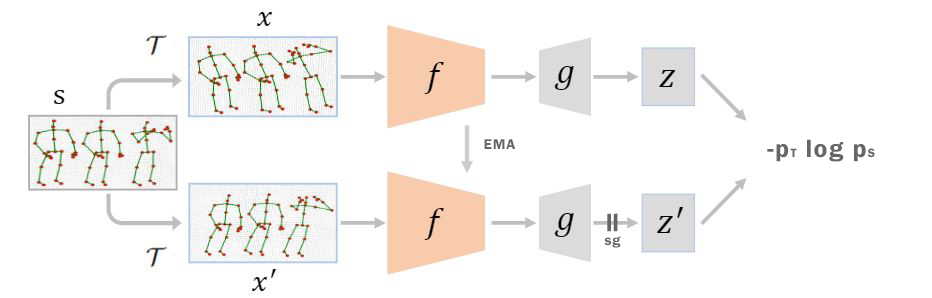
\includegraphics[width=.9\linewidth]{img/dino_illustrationv2.png}
	\caption{The output $h$ of the encoder $f$ go through a projection head $g$ to get embeddings $z$ and $z'$ for the student and the teacher, respectively .}\label{fig:dino_illustrationv2}
\end{figure}


\section{Second Approach Overview: PSTL \& ST-GCN}
The second approach in this study involves combining the "Partial Spatio-Temporal Learning" (PSTL) framework with the "Spatial Temporal Graph Convolutional Networks" (ST-GCN) as a backbone. This approach is motivated by the limitations of current contrastive learning-based methods in effectively leveraging the rich action clues stored in skeleton sequences. Current contrastive learning-based methods focus on finding effective global data augmentations to create various views of the skeleton. However, this global perspective may limit the model's ability to fully exploit the local relationships between different skeleton joints and video frames, especially in real-world scenarios. Moreover, these methods often require a large batch size or memory bank, making them unsuitable for scenarios with limited skeleton data. PSTL draws inspiration from the "Skeleton Barlow Twins" (SkeletonBT) method \cite{zbontar2021barlow}, which is known for its effective utilization of local relationships in skeleton sequences. Building on this idea, PSTL adopts a triple stream architecture, as shown in ~\ref{fig:pstl_pipline}. It applies Central Spatial Masking (CSM) on the spatial masking stream and Motion Attention Temporal Masking (MATM) on the temporal masking stream. Additionally, an extra anchor stream is included to retain the original semantic information.

\begin{figure}
	\centering
	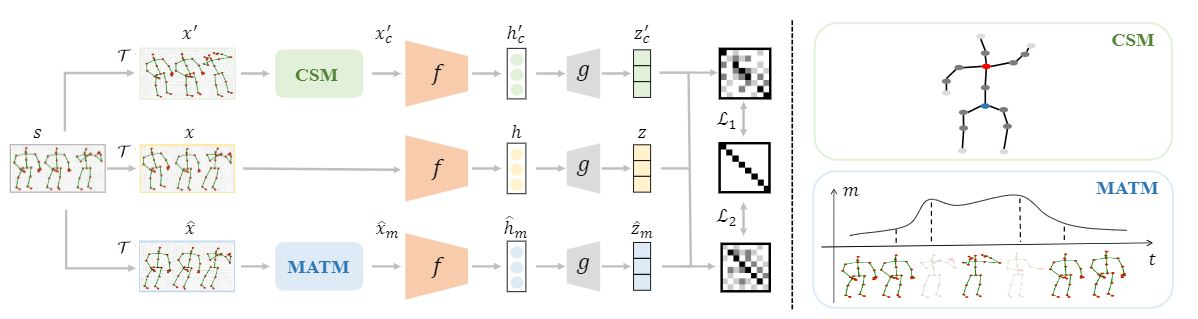
\includegraphics[width=.9\linewidth]{img/pstl_pipeline.JPG}
	\caption{ The general structure of PSTL representation in \cite{zhou2023self}.  Red, blue, dark gray, and light gray are the degrees for Central Spatial Masking (CSM). Motion Attention Temporal Mask (MATM) uses m to represent motion density and t to represent time.}\label{fig:pstl_pipline}
\end{figure}


Graph Convolution Networks (GCN) have demonstrated considerable success in the field of human action recognition. GCNs excel at processing data with graph structures, making them a suitable choice for handling skeleton-based action recognition tasks. The Spatial Temporal Graph Convolutional Networks (ST-GCN) model serves as the backbone for the PSTL framework. ST-GCN is capable of capturing both spatial and temporal dependencies within the skeleton sequences, and moreover, its stable results on different datasets make it well-suited for our study. The PSTL approach adopts a triple stream architecture, with all three streams utilizing the same encoder, which is the ST-GCN model. In the following section, each component of the ST-GCN model is described in detail. This includes a comprehensive explanation of how ST-GCN captures spatial and temporal information, processes graph structures, and extracts relevant features from skeleton sequences. By integrating the PSTL framework with the ST-GCN backbone, the second approach aims to overcome the limitations of current contrastive learning-based methods and enhance the model's performance and robustness in skeleton-based action recognition tasks. 

\subsection{Backbone Encoder: ST-GCN}
The Spatial Temporal Graph Convolutional Networks (ST-GCN) is a powerful model designed for action recognition tasks, specifically tailored for skeleton-based data. The motivation behind using graph convolution networks arises from the fact that skeletons are inherently represented in the form of graphs, where each node corresponds to a joint of the human body. This graph representation makes it challenging to utilize traditional models like convolutional networks, which are designed for 2D or 3D grids. The ST-GCN model is formulated on top of a sequence of skeleton graphs, where each graph represents a single frame of the action sequence. The graph nodes represent the joints of the human body, while the edges can be of two types: spatial edges that encode the natural connectivity of joints within the human body structure, and temporal edges that connect the same joints across consecutive timesteps in the action sequence, as shown in ~\ref{fig:STGCN_Illustration}. The core of the ST-GCN model lies in the construction of multiple layers of spatial temporal graph convolution. These layers enable the integration of information along both the spatial and temporal dimensions of the skeleton data. This integration allows the model to capture the spatial relationships between joints in a single frame as well as the temporal dependencies between corresponding joints across consecutive frames in the action sequence.

\begin{figure}
	\centering
	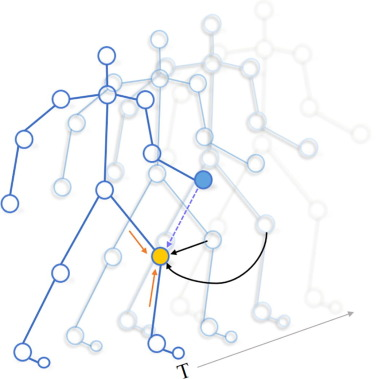
\includegraphics[width=.4\linewidth]{img/STGCN_Illustration.jpg}
	\caption{Illustration in \cite{peng2021rethinking} of modeling skeleton with ST-GCNs.}\label{fig:STGCN_Illustration}
\end{figure}

In ST-GCN, the graph denoted as $G = (V, E)$ is formed on a skeleton sequence with $N$ joints and $T$ frames, capturing both intra-body and inter-frame connections. The node set $V = \{v_{ti} \| t = 1,...,T,i=1,...,N\}$ includes all the joints in the skeleton sequence. The input to the ST-GCN model is represented by the feature vector on each node $F(v_{ti})$, which comprises the coordinate vectors and estimation confidence of the $i$-th joint on frame $t$. To construct the spatial temporal graph, the model perform the process in two steps:

\textbf{Intra-Skeleton Connection (Spatial Edges):} Within each frame, the joints are connected based on the natural connectivity of the human body structure. These connections, denoted as $E_S = \{v_{ti} v_{tj} \| (i,j) \in H\}$, are established using the set $H$, which specifies the naturally connected human body joints. This automatic assignment of connections ensures that the network architecture can handle datasets with varying numbers of joints or joint connectivities.

\textbf{Inter-Frame Connection (Temporal Edges):} Each joint is connected to the corresponding joint in the consecutive frame, forming inter-frame edges denoted as $E_F =\{v_{ti} v_{(t+1)i}\}$.
These inter-frame edges capture the temporal relationships and represent the trajectories of each joint over time. Thus, for a given joint $i$, all edges in $E_F$ will indicate its trajectory through time.

Spatial Graph Convolution allows the model to perform convolutional operations on the spatial graph, treating each frame independently and encoding the relationships between joints within a single frame. Let's delve into the details of the Spatial Graph Convolution. In this case, on a single frame at time $\tau$, we have $N$ joint nodes $V_t$, and the skeleton edges $E_S = \{v_{ti} v_{tj} \| t = \tau, (i,j) \in H$ represent the connectivity between joints based on the human body structure. The convolution operation on graphs is an extension of the traditional 2D convolution on regular grids. Let's denote the input feature map on the spatial graph as $f^t_{in} : V_t \to \mathbb{R}^c$, where $c$ is the number of channels or dimensions of the feature vectors on each node. The output feature map $f_{out}$  is computed by summing over the sampled input features from neighboring nodes on the graph, multiplied by learnable weight vectors $w(l_{ti}(v_{tj}$ associated with each sampled input feature:

$$
f_{o u t}\left(v_{t i}\right)=\sum_{v_{t j} \in B\left(v_{t i}\right)} \frac{1}{Z_{t i}\left(v_{t j}\right)} f_{i n}\left(v_{t j}\right) \cdot \mathbf{w}\left(l_{t i}\left(v_{t j}\right)\right)
$$

\begin{itemize}
	\item $f_{out}(v_{ti})$ is the output feature at node $v_{ti}$
	\item $B(v_{ti})$ is the set of neighboring nodes of $v_{ti}$
	\item $Z_{ti}(v_{tj})$ is a normalization factor for the sampled features, and 
	\item $\mathbf{w}(l_{ti}(v_{tj}))$  is a learnable weight vector associated with each sampled input feature.
\end{itemize}

This formulation allows the ST-GCN model to perform graph convolutions efficiently on spatial graphs, treating each frame independently and considering the spatial relationships between different joints within a single frame. It provides a graph-based alternative to standard 2D convolutions and enables the model to effectively handle skeletal data for action recognition tasks.

\subsection{Learning Strategy: PSTL}
The Partial Spatio-Temporal Learning (PSTL) framework presents an innovative approach to exploit local relationships from a partial skeleton sequence using a unique spatio-temporal masking strategy. The motivation behind PSTL is to address the limitations of existing contrastive learning-based methods that often rely heavily on strong data augmentation strategies, which may neglect the rich action clues stored in the skeleton sequences. The PSTL framework is built upon a triplet stream structure, which includes an anchor stream, a spatial masking stream with Central Spatial Masking (CSM), and a temporal masking stream with Motion Attention Temporal Masking (MATM), as shown in ~\ref{fig:pstl_pipline}. In each stream, ordinary augmentations are initially applied to enhance the diversity of input samples.

A 3D human skeleton sequence is denoted as \(s \in \mathbb{R}^{C \times T \times V}\), where \(T\) represents the number of frames and \(V\) denotes the number of joints. The channel dimension \(C\) represents the 3D position of the skeleton. To start the self-supervised learning process, the input skeletons are first augmented using an ordinary augmentation function $\Tau$ to obtain diverse views \(x\) and \(x'\).

Next, an encoder \(f\) is utilized to extract features \(h = f(x;\theta)\) and \(h' = f(x';\theta)\), where \(h, h' \in \mathbb{R}^{c_h}\), and \(\theta\) represents the encoder's parameters. Following the feature extraction, a projector \(g\) maps each feature to a higher-dimensional space, generating embeddings \(z = g(h)\) and \(z' = g(h')\), where \(z, z' \in \mathbb{R}^{c_z}\).

The core objective of PSTL is to encourage the empirical cross-correlation matrix \(\mathcal{C}\) between embeddings \(z\) and \(z'\) to approximate an identity matrix, thereby capturing the relationship between the two streams. To achieve this, PSTL employs the following loss function:

\[
\mathcal{L} = \sum_i \left(1 - \mathcal{C}_{ii}\right)^2 + \lambda \sum_i \sum_{j \neq i} \mathcal{C}_{ij}^2
\]

where \(\mathcal{C}\) is the cross-correlation matrix computed between embeddings \(z\) and \(z'\) along the batch dimension \(b\):

\[
\mathcal{C}_{ij} = \frac{\sum_b z_{b,i} z_{b,j}'}{\sqrt{\sum_b\left(z_{b,i}\right)^2} \sqrt{\sum_b\left(z_{b,j}'\right)^2}}
\]

In this loss function, the first term encourages the diagonal elements of \(\mathcal{C}\) to be close to 1, making the embeddings invariant to the applied augmentation. The second term forces the off-diagonal elements of \(\mathcal{C}\) to be close to 0, effectively decoupling different embedding components to minimize redundancy within the representation. The trade-off parameter \(\lambda\) balances the contribution of the two terms.

By minimizing the loss \(\mathcal{L}\), PSTL encourages the encoder to capture meaningful relationships between different streams of the augmented skeletons, resulting in discriminative and robust representations that can be effectively used for downstream tasks like action recognition.

The traditional approach of directly setting the values of masked joints to zero is unreasonable for skeleton data, as it removes the joint semantic information, which is critical for action recognition. In the spatial masking stream, \textit{Central Spatial Masking (CSM)} is used to filter out selected joints from the feature calculation process. Instead of setting the selected joint positions to zeros, which may not be suitable for skeleton data, the approach considers the topology of the human skeleton as a predefined graph. By filtering out joints with higher probabilities of centrality, the encoder can focus more on less explored skeletons, enhancing the model's understanding of the joints' connectivity.

To further improve the strategy, the concept of degree centrality in the human skeleton graph topology is leveraged. It is observed that joints with higher degrees (more connected) can acquire richer neighborhood information. Thus, CSM assigns higher probabilities to mask joints that have more connectivity. By masking such connected joints, the encoder can capture relationships between a wider range of joint information.

The process of assigning masked probabilities is as follows: Let \(V_i\) denote the \(i\)-th joint in the skeleton, where \(i \in (1, 2, ..., n)\), and \(n\) is the total number of joints in the skeleton. There are four types of joints: light gray joints located at the margin of the graph have a degree of 1, dark gray joints have a degree of 2 (more connective and the majority in the graph), blue joints have a degree of 3, and red joints have a degree of 4, as shown in ~\ref{fig:pstl_pipline}.

To calculate the masked probability for each joint \(V_i\), the degree \(d_i\) of each joint is first computed, and then the probability \(p_i\) is set as follows:

\[ p_i = \frac{d_i}{\sum_{j=1}^n d_j} \]

where \(d_i\) represents the degree of the \(i\)-th joint, and the denominator \(\sum_{j=1}^n d_j\) ensures that the probabilities sum up to 1. By using this strategy, CSM focuses on masking joints based on their degree centrality, enhancing the encoder's ability to capture a broader range of joint relationships.

In the temporal masking stream, the \textit{Motion Attention Temporal Masking (MATM)} strategy is introduced to prioritize frames that change quickly. These frames often contain more semantic information about the actions, making them more valuable for learning meaningful representations. To compute the motion \(m \in \mathbb{R}^{C \times T \times V}\) of the sequences, the temporal displacement between frames is calculated as \(m_{:,t,:} = x_{:,t+1,:} - x_{:,t,:}\), where \(x\) is the input skeleton sequence with \(T\) frames and \(V\) joints.

Next, MATM calculates the overall motion rate of a frame, which serves as the attention weight. The motion rate \(a_t\) for frame \(t\) is computed as follows:

\[ a_t = \frac{(m_t)^2}{\sum_{i=1}^T (m_i)^2} \]

where \(a_t\) represents the motion rate of frame \(t\), and the denominator \(\sum_{i=1}^T (m_i)^2\) ensures that the attention weights sum up to 1.

Once the attention weights are computed, the top-K attention weights \(a_{t1}, ..., a_{t_K}\) are selected, and the corresponding frames \(x_{t_1}, ..., x_{t_K}\) serve as the key-frames that contain more semantic information about the actions. These key-frames are then masked, and the encoder is encouraged to capture the relationship between the feature from the masked sequence and the anchor feature, which contains the total semantic information.

To capture the relationship between masked joints and unmasked ones, two cross-correlation matrices \(\mathcal{C}'\) and \(\hat{\mathcal{C}}\) are computed between embeddings \(z\) and \(z'_c\), and between \(z\) and \(\hat{z}_m\), respectively. These cross-correlation matrices are used to formulate the loss functions \(\mathcal{L}_1\) and \(\mathcal{L}_2\), which help in guiding the encoder to learn meaningful and discriminative representations.

The loss function \(\mathcal{L}_1\) is formulated as follows:

\[ \mathcal{L}_1 = \sum_i \left(1 - \mathcal{C}_{ii}'\right)^2 + \lambda \sum_i \sum_{j \neq i} \left(\mathcal{C}_{ij}'\right)^2 \]

The first term of \(\mathcal{L}_1\) encourages the diagonal elements of \(\mathcal{C}'\) to be close to 1, forcing the representation of the partial data to be similar to that of the total data. The second term promotes the decoupling of different embedding components, minimizing redundancy within the representation and preventing it from becoming a constant.

Similarly, the cross-correlation matrix \(\hat{\mathcal{C}}\) between \(z\) and \(\hat{z}_m\) is used to formulate the loss function \(\mathcal{L}_2\):

\[ \mathcal{L}_2 = \sum_i \left(1 - \hat{\mathcal{C}}_{ii}\right)^2 + \lambda \sum_i \sum_{j \neq i} \left(\hat{\mathcal{C}}_{ij}\right)^2 \]

The loss \(\mathcal{L}_2\) captures the relationship between masked and unmasked frames. The trade-off parameter \(\lambda\) is used to balance the dimension difference between the first and second terms, keeping the same weight on both losses.

The total loss \(\mathcal{L}\) for PSTL is then given by:

\[ \mathcal{L} = \mathcal{L}_1 + \mathcal{L}_2 \]

By optimizing this total loss, PSTL encourages the encoder to learn meaningful and robust representations that capture both spatial and temporal relationships within the skeleton sequences, leading to improved performance on downstream action recognition tasks.


At the conclusion of this chapter, we presented two different approaches as our methodology to address the challenge of recognizing human actions based on skeleton data using self-supervised learning. The first approach utilizes the DINO framework, originally designed for images, and adapts it to skeleton data by employing the STTFormer as the backbone. The DINO approach employs self-distillation with no labels, enabling the student network to learn from the teacher network's predictions. On the other hand, the second approach leverages the Partial Spatio-Temporal Learning (PSTL) framework in combination with the ST-GCN backbone. PSTL employs a unique spatio-temporal masking strategy to exploit the local relationships between skeleton joints and frames. By investigating these two distinct solutions, we aim to tackle the research question of recognizing human actions from skeleton data through self-supervised learning. The comparison between DINO with STTFormer and ST-GCN with PSTL will provide valuable insights into the efficacy and suitability of each approach for skeleton-based action recognition, paving the way for further advancements in self-supervised learning in the context of human action understanding.